% Options for packages loaded elsewhere
\PassOptionsToPackage{unicode}{hyperref}
\PassOptionsToPackage{hyphens}{url}
%
\documentclass[
]{article}
\usepackage{amsmath,amssymb}
\usepackage{lmodern}
\usepackage{iftex}
\ifPDFTeX
\usepackage[T1]{fontenc}
\usepackage[utf8]{inputenc}
\usepackage{textcomp} % provide euro and other symbols
\else % if luatex or xetex
\usepackage{unicode-math}
\defaultfontfeatures{Scale=MatchLowercase}
\defaultfontfeatures[\rmfamily]{Ligatures=TeX,Scale=1}
\fi
% Use upquote if available, for straight quotes in verbatim environments
\IfFileExists{upquote.sty}{\usepackage{upquote}}{}
\IfFileExists{microtype.sty}{% use microtype if available
	\usepackage[]{microtype}
	\UseMicrotypeSet[protrusion]{basicmath} % disable protrusion for tt fonts
}{}
\makeatletter
\@ifundefined{KOMAClassName}{% if non-KOMA class
	\IfFileExists{parskip.sty}{%
		\usepackage{parskip}
	}{% else
		\setlength{\parindent}{0pt}
		\setlength{\parskip}{6pt plus 2pt minus 1pt}}
}{% if KOMA class
	\KOMAoptions{parskip=half}}
\makeatother
\usepackage{xcolor}
\IfFileExists{xurl.sty}{\usepackage{xurl}}{} % add URL line breaks if available
\IfFileExists{bookmark.sty}{\usepackage{bookmark}}{\usepackage{hyperref}}
\hypersetup{
		pdftitle={Central Limit Theorem},
			pdfauthor={Anthony Perez Eisenbarth},
						hidelinks,
		pdfcreator={LaTeX via pandoc}}
\urlstyle{same} % disable monospaced font for URLs
\usepackage[margin=3cm]{geometry}
\usepackage{graphicx}
\makeatletter
\def\maxwidth{\ifdim\Gin@nat@width>\linewidth\linewidth\else\Gin@nat@width\fi}
\def\maxheight{\ifdim\Gin@nat@height>\textheight\textheight\else\Gin@nat@height\fi}
\makeatother
% Scale images if necessary, so that they will not overflow the page
% margins by default, and it is still possible to overwrite the defaults
% using explicit options in \includegraphics[width, height, ...]{}
\setkeys{Gin}{width=\maxwidth,height=\maxheight,keepaspectratio}
% Set default figure placement to htbp
\makeatletter
\def\fps@figure{htbp}
\makeatother
\setlength{\emergencystretch}{3em} % prevent overfull lines
\providecommand{\tightlist}{%
	\setlength{\itemsep}{0pt}\setlength{\parskip}{0pt}}
\setcounter{secnumdepth}{-\maxdimen} % remove section numbering
\usepackage{hyperref}
\usepackage{array}
\usepackage{caption}
\usepackage[flushleft]{threeparttable}
\usepackage[sfdefault, condensed]{roboto}
\ifLuaTeX
\usepackage{selnolig}  % disable illegal ligatures
\fi

\title{Central Limit Theorem}
\author{Anthony Perez Eisenbarth}
\date{}

\begin{document}
				\maketitle
				
							The Central Limit Theorem (CLT) establishes that, when
       independent random variables are added, their properly normalized
       sum tends toward a normal distribution (informally a bell curve)
       even if the original variables themselves are not normally
       distributed. Put another way, the CLT states that the sum of a
       number of independent and identically distributed random
       variables with finite variances will tend to a normal
       distribution as the number of variables grows.

       A simple example of this is that if one flips a coin many times,
       the probability of getting a given number of heads will approach
       a normal distribution, with the mean equal to half the total
       number of flips. At the limit of an infinite number of flips, it
       will equal a normal distribution.

       In this experiment, \(m = 1000\) random samples are produced,
       each of which with \(n = 40\) observations. All the observations
       were produced from an exponential distribution
       \(\lambda e^{-\lambda x}\) with rate \(\lambda = 0.2\). The goal
       of the experiment is verify, through simulation, the veracity of
       the CLT. If the CLT holds, then the probability distribution of
       the average and the variance of the samples drawn from the above
       exponential distribution will converge to a standard normal
       distribution.

       \hypertarget{simulated-samples}{%
       \section{Simulated Samples}\label{simulated-samples}}

       From the simulation, a 1000 samples \(\underline{y}_i\) were
       obtained, which contain observations that are the realizations of
       the 40000 i.i.d. random variables \(Y_{i,j} \sim Exp(0.2)\) where
       \(i = 1,2,\dots,1000\) and \(j = 1,2, \dots 40\). A random
       variable \(Y_{i,j} \sim Exp(\lambda)\), where
       \(\lambda \in (0, \infty)\), has an expected value
       \(\mu_Y := E(Y_{i,j}) = \frac{1}{\lambda}\)and variance
       \(\sigma_Y^2 := Var(Y_{i,j}) = \frac{1}{\lambda^2}\). So for
       \(\lambda = 0.2\) it is \(\mu_{Y} = 5\) and \(\sigma_Y^2 = 25\).

       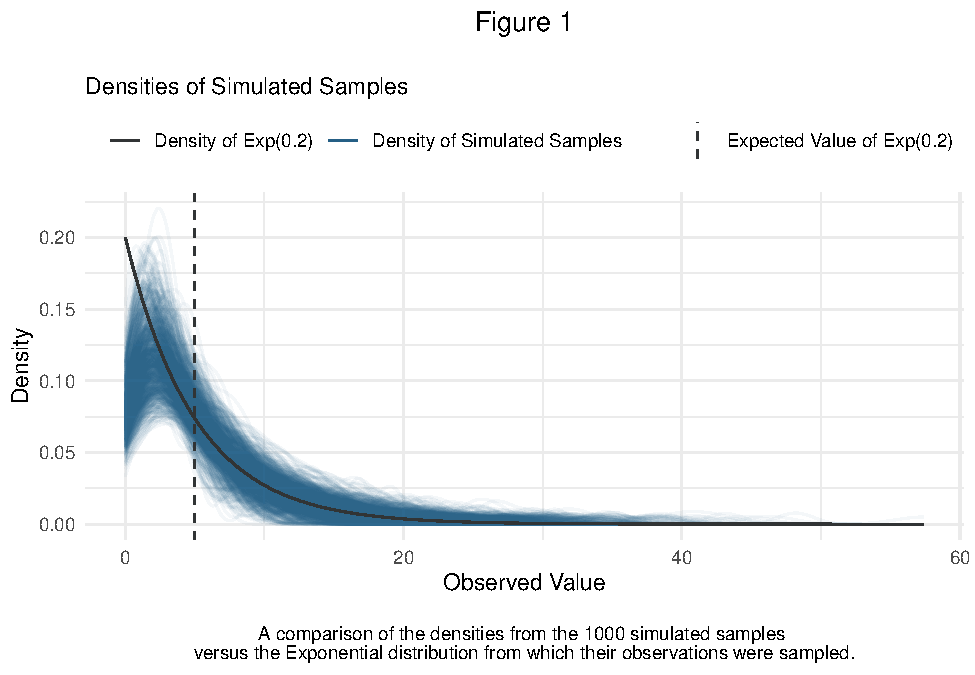
\includegraphics{CLT_files/figure-latex/unnamed-chunk-4-1.pdf}

       \hypertarget{sample-of-sample-means}{%
       \section{Sample of Sample Means}\label{sample-of-sample-means}}

       For each random sample
       \(\underline{Y}_i = (Y_{i,1}, Y_{i,2}, \dots, Y_{i,40})\), the
       random variable
       \(\bar{Y}_i = \frac{1}{40} \cdot \sum_{j = 1}^{40} Y_{ij}\),is
       the sampling mean. The sampling means \(\bar{Y}_i\), of the the
       1000 random samples, are i.i.d. random variables because they are
       linear transformations of the i.i.d. random variables
       \(Y_{i,j}\).

       Define \(X_i:=\bar{Y_i}\), so the random variable \(X_i\) has
       expected value \(\mu_X = E(X_i) = E(\bar{Y}_i)\) and variance
       \(\sigma_X^2 = Var(X_i) = Var(\bar{Y}_i)\). The sample
       \(\underline{x} = (x_1, x_2, \dots, x_{1000}) \equiv (\bar{y}_1, \bar{y}_2, \dots, \bar{y}_{1000})\)
       where
       \(x_i = \bar{y}_i = \frac{1}{40} \cdot \sum_{j = 1}^{40} y_{i,j}\),
       consists of the observed sample means of 1000 original samples
       \(\underline{y}_1, \underline{y}_2, \dots, \underline{y}_{1000}\)

       \hypertarget{mean-of-sample-means}{%
       \section{Mean of Sample Means}\label{mean-of-sample-means}}

       According to the proposition (P1), the random variable \(X_i\)
       defined as equivalent to the sampling mean \(\bar{Y}_i\) of the
       i-th random sample with \(n\) observations, has an expected value
       equal to the expected value of the distribution from which the
       sample was taken.

       So \(\mu_{X} = E(X_i) = E(\bar{Y_i}) = E(Y_{ij}) = \mu_{Y} = 5\).

       Indeed the mean \(\bar{x} = 4.992119\), of the sample
       \(\underline{x}\), is `very close' to the theoretical expected
       value \(\mu_X = 5\).

\begin{verbatim}
## [1] 4.992119
\end{verbatim}

       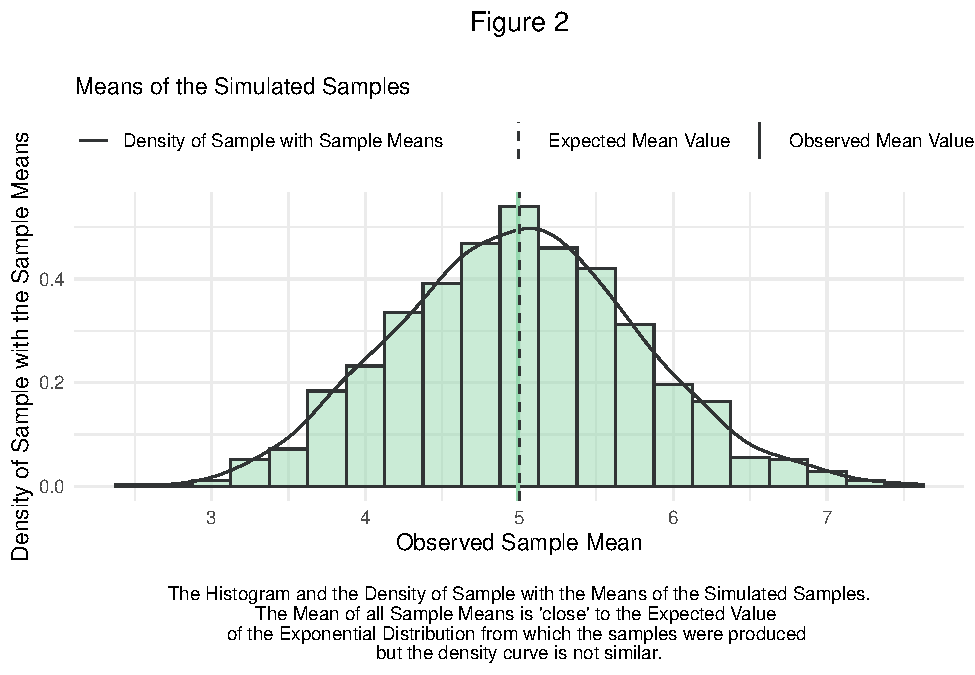
\includegraphics{CLT_files/figure-latex/unnamed-chunk-8-1.pdf}

       Furthermore as the number of means from sample means increases
       the cumulative mean converges to the expected value \(\mu_x = 5\)
       (Figure 3).

       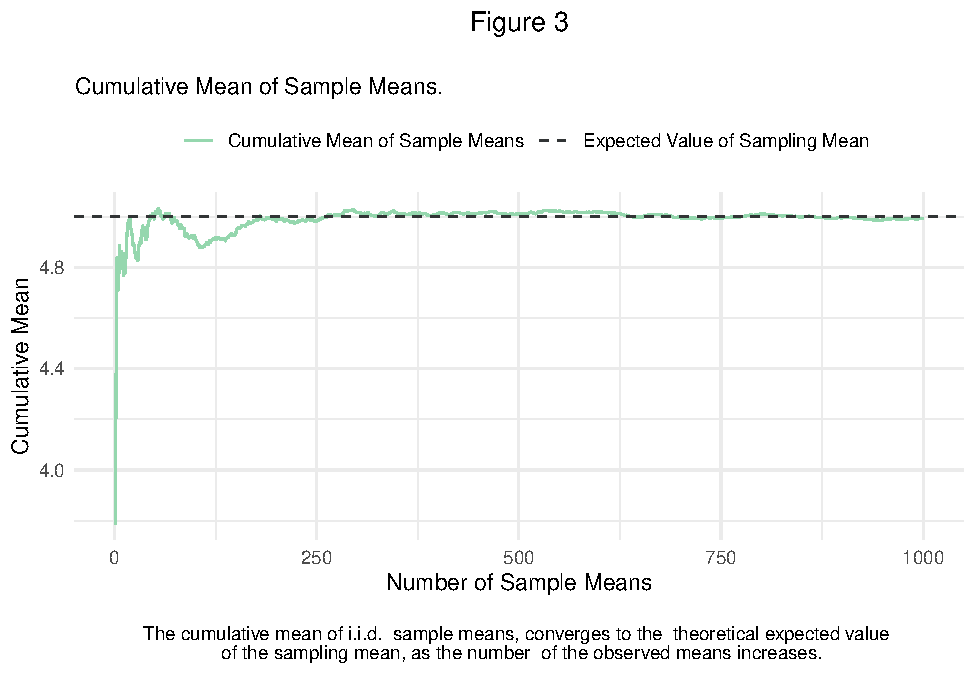
\includegraphics{CLT_files/figure-latex/unnamed-chunk-9-1.pdf}

       \hypertarget{variance-of-sample-means}{%
       \section{Variance of Sample
       Means}\label{variance-of-sample-means}}

       According to the proposition (P2), the random variable \(X_i\)
       defined as equivalent to the sampling mean \(\bar{Y}_i\) of the
       i-th random sample with \(n\) observations, has a variance equal
       to the variance of the distribution from which the sample was
       taken divided by the sample size \(n\).

       So
       \(\sigma_X^2 = Var(X_i) = Var(\bar{Y_i}) = \frac{Var(Y_{ij})}{n} = \frac{\sigma_Y^2}{n} = 0.625\).

       Indeed the sample variance \(s^2 = 0.625151\), of the sample
       \(\underline{x}\), is `very close' to the theoretical variance
       \(\sigma_X^2 = 0.625\).

\begin{verbatim}
## [1] 0.625151
\end{verbatim}

       Furthermore as the number of means from sample means increases
       the cumulative variance converges to the expected value
       \(\sigma_X^2 = 5\) (Figure 4).

       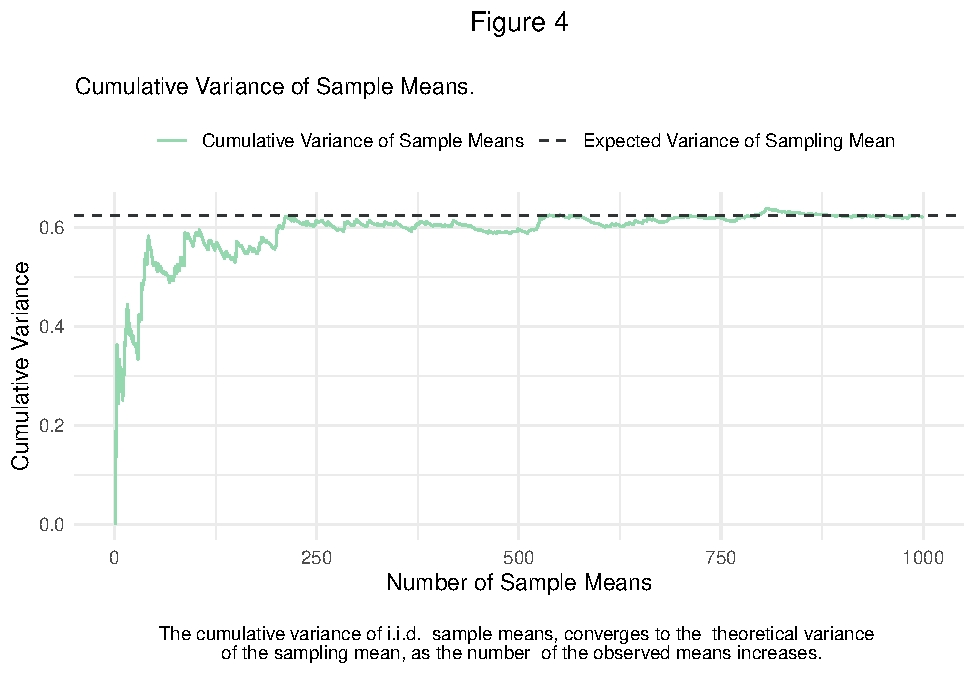
\includegraphics{CLT_files/figure-latex/unnamed-chunk-12-1.pdf}
       \newpage

       \hypertarget{distribution-of-sample-means}{%
       \section{Distribution of Sample
       Means}\label{distribution-of-sample-means}}

       According to the proposition (P3), the distribution of the random
       variable \(X_i\) defined as equivalent to the sampling mean
       \(\bar{Y}_i\) of the i-th random sample with n observations, is
       approximately Normal with expected value \(\mu_X\) and variance
       \(\sigma_X^2\).

       From a visual examination of the density (Figure 5), and the QQ
       plot (Figure 6) of the sample \(\underline{x}\) with the means of
       the simulated samples it is clear that the observed values fit or
       approximate those from a normal distribution with expected value
       \(\mu_X = 5\) and variance \(\sigma_X^2 = 0.625\).

       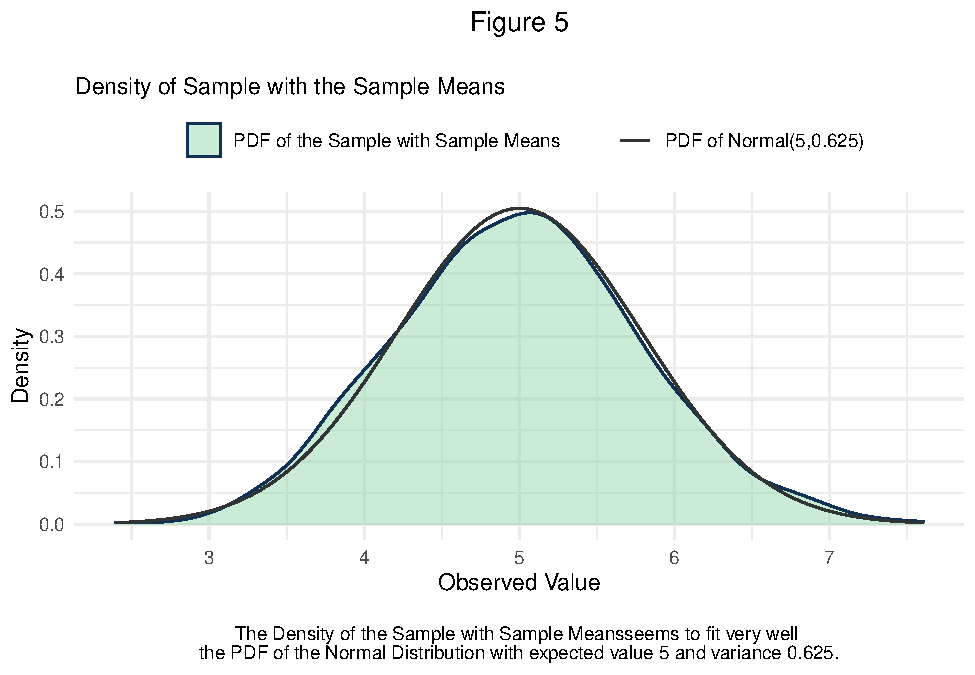
\includegraphics{CLT_files/figure-latex/unnamed-chunk-13-1.pdf}

       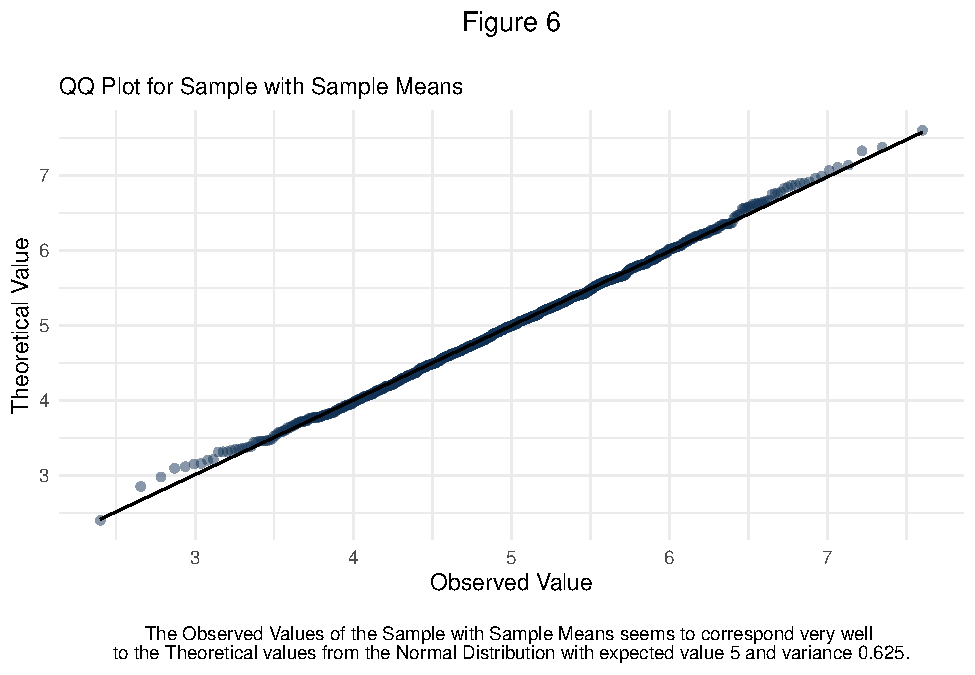
\includegraphics{CLT_files/figure-latex/unnamed-chunk-14-1.pdf}

       The normality assumption was also verified with the Shapiro-Wilk
       test, from which a p-value 0.680 was obtained, indicating that
       there are not enough evidence to discard the null hypothesis,
       that the sample comes from a Normal Distribution.

\begin{verbatim}
## 
##  Shapiro-Wilk normality test
## 
## data:  sample_means$value
## W = 0.99869, p-value = 0.6803
\end{verbatim}

       \hypertarget{remarks}{%
       \section{Remarks}\label{remarks}}

       It is quite possible, especially for the proposition (P3), to
       obtain samples that may not pass the Shapiro-Wilk test for
       normality. By increasing the number of simulated samples and/or
       the sample size of each of them, the observations will eventually
       conform with the claims of Central Limit Theorem (CTL) and the
       Law of Large Numbers (LLN).
	
				\end{document}